\documentclass[c]{beamer}
\usepackage[italian]{babel}
\defbeamertemplate{description item}{align left}{\insertdescriptionitem\hfill}
\setbeamertemplate{description item}[align left]

\usetheme{CambridgeUS}

\title[GraphQL e Model Driven Programming]{Sviluppo di un generatore di codice per librerie ORM SQL basato su schemi GraphQL}

\newsavebox{\authbox}
\sbox{\authbox}{%
    \centering
    \begin{minipage}{0.45\linewidth}
    \centering\normalsize
    Candidato \par
    Ivan Perazzini
    \end{minipage}
    \hfill
    \begin{minipage}{0.45\linewidth}
    \centering\normalsize
    Relatore \par
    prof. Mirko Viroli
    \end{minipage}
}

\author[Ivan Perazzini]{\texorpdfstring{\usebox{\authbox}}{}}

\institute[Università di Bologna]{Ingegneria e Scienze Informatiche\\Alma Mater Studiorum—Università di Bologna, Cesena}
\date{\today}
\begin{document}
    \begin{frame}
        \titlepage
    \end{frame}

    \begin{frame}
        \frametitle{Outline}
        \tableofcontents
    \end{frame}
    \section{Introduzione}
        \begin{frame}
            \frametitle{Twinlogix}
            \emph{Twinlogix S.r.l}, azienda di Santarcangelo di Romagna, ha post fra gli obiettivi interni il passaggio completo da API Rest a GraphQL.
            \vfill
            Sta anche pensando di sfruttare le potenzialità del linguaggio GraphQL per costruire strumenti di generazione di codice basati su di esso.
            \vfill
            L'obiettivo di questa tesi sarà studiare ed implementare una versione del generatore per database SQL.
        \end{frame}
    \section{GraphQL}
        \subsection{Storia}
            \begin{frame}
                \frametitle{GraphQL}
                È un linguaggio per API ideato per descrivere operazione di lettura e scrittura di dati definito da Facebook nel 2012 ed dal 2018 diventato standard gestito da \emph{GraphQL Foundation}.
                \begin{itemize}
                    \item i dati gestiti da Facebook come post, utenti, commenti e reazioni risultano meglio rappresentabili da database non relazionali;
                    \item allo stesso tempo, il valore di questi dati risiede nelle relazioni fra di essi (adesempio, quali utenti sono amici di altri);
                    \item i database relazionali (in questo caso, documentali) non presentano nativamente meccanismi di relazione fra documenti diversi;
                    \item non esiste un linguaggio di querying unificato per database NoSQL.
                \end{itemize}
            \end{frame}

        \subsection{Caratteristiche}
            \begin{frame}
                Il linguaggio GraphQL permette di definire uno schema costituito da:
                \vfill
                \begin{description}[align left]
                    \item[Oggetti] Struttura delle entità gestite dall'applicazione, composte da campi tipizzati.
                    \begin{figure}
                        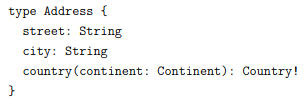
\includegraphics[height=0.2\textheight]{GraphQL_obj.png}
                    \end{figure}
                    \item[Query e mutazioni] Operazioni di lettura e scrittura esposte al client.
                    \begin{figure}
                        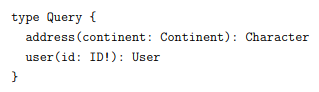
\includegraphics[height=0.2\textheight]{GraphQL_query.png}
                    \end{figure}
                \end{description}
                \vfill
                Per arricchire l'espressività dello schema è possibile usare \emph{direttive}, parole chiave definite nello schema.
            \end{frame}
    
    \section{Progetto}
        \subsection{Architettura}
            \begin{frame}
                \begin{columns}
                    \frametitle{Architettura del progetto}
                    \column{0.4\textwidth}
                        Per la generazione del codice è stato scritto un plugin per l'applicativo \emph{GraphQL code generator} composto da:
                        \begin{itemize}
                            \item un modulo \emph{visitor} per elaborare tipi ed interfacce dello schema;
                            \item un modulo per controllare l'integrità dei tipi rielaborati;
                            \item un generatore per gli schemi del database;
                            \item un generatore per i DAO.
                        \end{itemize}
                    \column{0.6\textwidth}
                        \begin{figure}
                            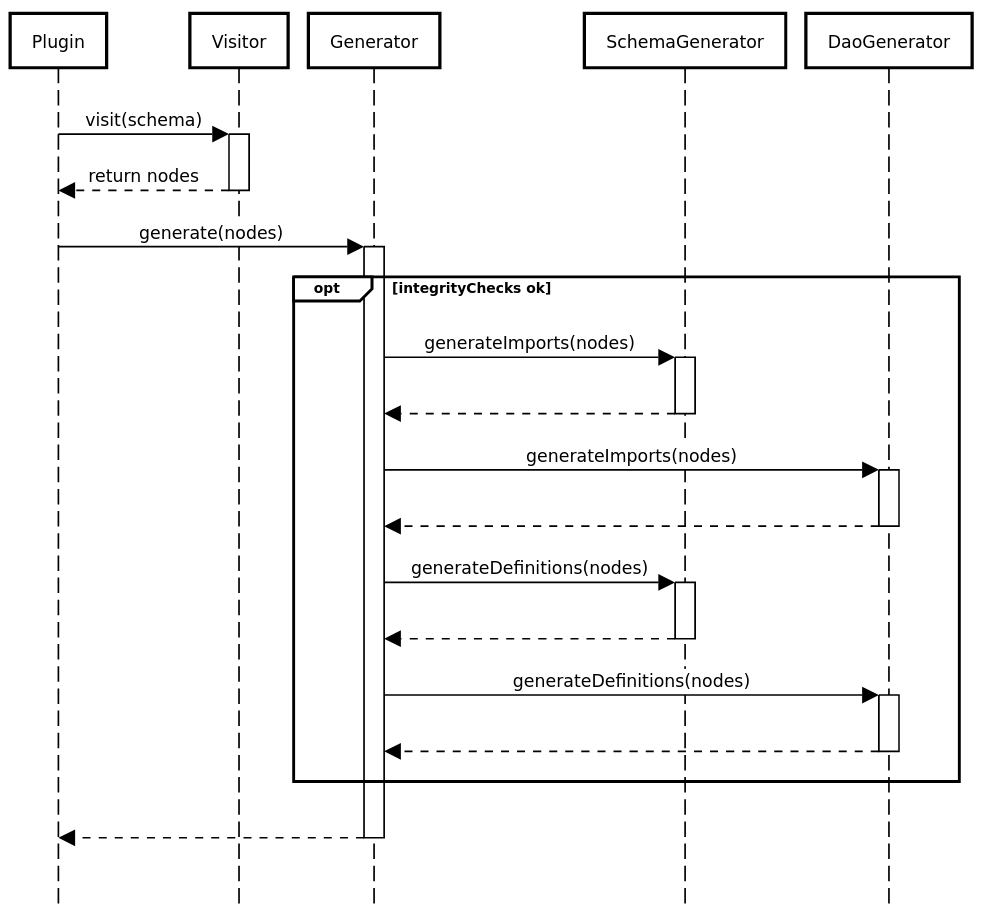
\includegraphics[scale=0.2]{../generator_workflow.png}
                        \end{figure}
                \end{columns}
            \end{frame}

            \begin{frame}
                \begin{figure}
                    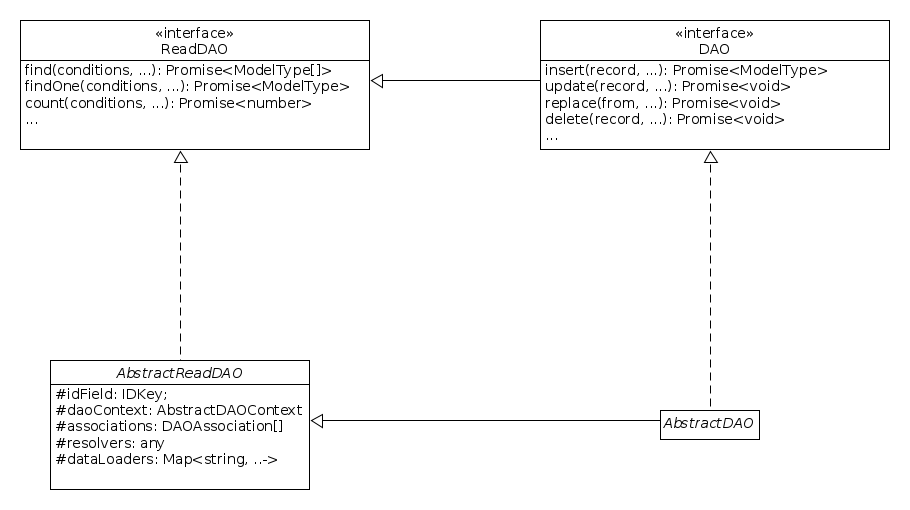
\includegraphics[scale=0.26]{../prototype-architecture.png}
                \end{figure}
                Per gestire l'interazione con le entità generate l'azienda ha impiegato il pattern \emph{Data Access Object}, definendo un DAO generico.
                \vfill
                Le implementazioni astratte di questo DAO si occupano di effettuare le operazioni su Database, interfacciandosi con driver e librerie apposite.
            \end{frame}

        \subsection{Obiettivi}
            \begin{frame}
                \frametitle{Esempi di funzionamento}
                Una volta generati i modelli delle tabelle, i DAO e i tipi di supporto al tipo di dato (filtri, proiezioni e ordinamenti), i DAO generati possono svolgere
                operazioni sulle tabelle del database.
                \begin{columns}[T]
                    \column{0.45\textwidth}
                        \begin{figure}
                            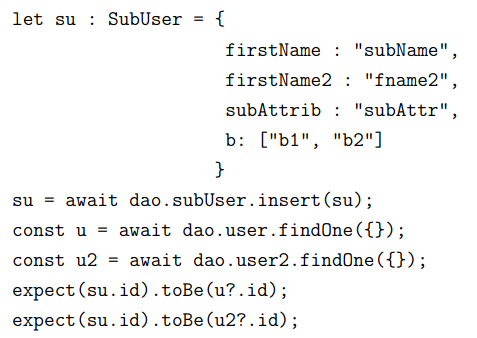
\includegraphics[scale=0.4]{Example_Insert.png}
                            \caption{Esempio di inserimento}
                        \end{figure}
                    \column{0.55\textwidth}
                        \begin{figure}
                            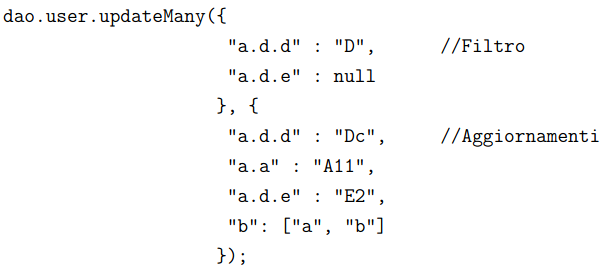
\includegraphics[scale=0.4]{Example_Update.png}
                            \caption{Esempio di aggiornamento}
                        \end{figure}
                \end{columns}
            \end{frame}

        \subsection{Svolgimento}
            \begin{frame}
                \frametitle{Soluzione adottata - alto livello}
                \begin{columns}
                    \column{0.28\textwidth}
                    \begin{figure}
                        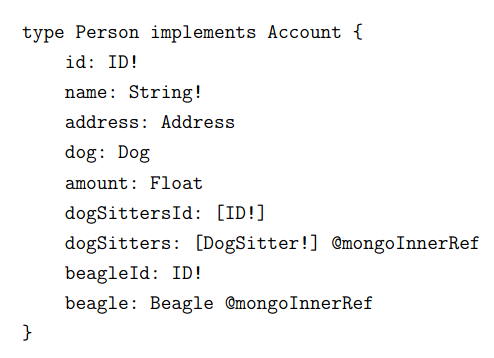
\includegraphics[scale=0.28]{Tipo_difficile.png}
                    \end{figure}
                    \column{0.72\textwidth}
                    \begin{figure}
                        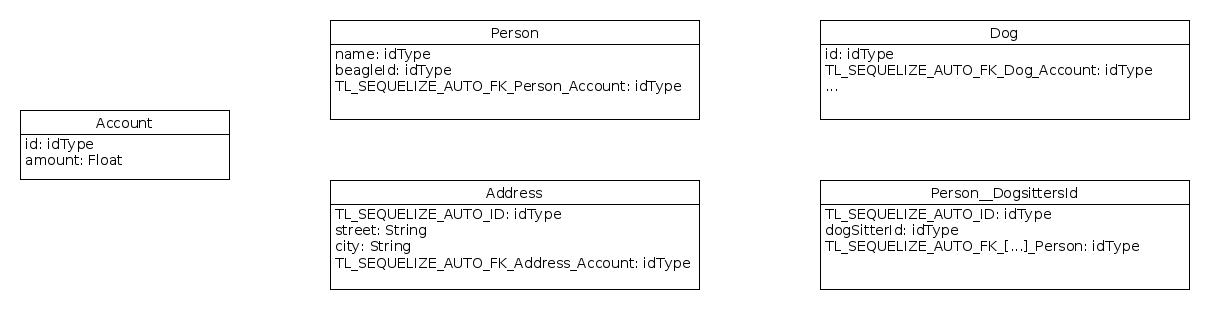
\includegraphics[scale=0.24]{../db-example.jpg}
                    \end{figure}
                \end{columns}
                \vfill
                Le entità composte o implementanti interfacce sono gestite tenendo i campi comuni nelle tabelle delle interfacce e creando tabelle secondarie per array e tipi embedded.
            \end{frame}

            \begin{frame}
                \frametitle{Soluzione adottata - implementazione}
                Per la gestione della connessione e operazioni su db, è stata usata la libreria ORM Sequelize.
                \vfill
                Le gerarchie e le composizioni sono modellate tramite le \emph{associations} di Sequelize.
                Ogni DAO conserva al suo interno una mappa che associa nomi di campi ad associazioni.
                \begin{figure}
                    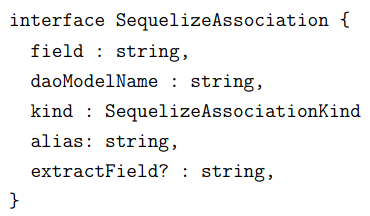
\includegraphics[scale=.5]{Sequelize_assoc.png}
                \end{figure}
            \end{frame}

            \begin{frame}
                Se durante una operazione vengono rilevati campi appartenenti ad una associazione, la gestione dell'operazione su quei campi
                è delegata ai DAO di competenza.
                \begin{figure}
                    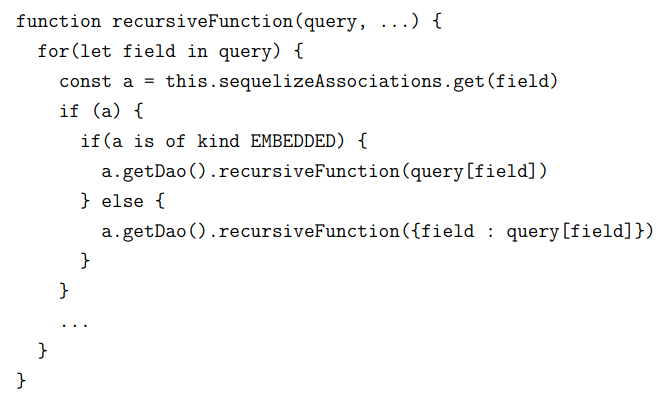
\includegraphics[scale=.5]{Resolution_Example.png}
                    \caption{Struttura tipo dei metodi del DAO}
                \end{figure}
            \end{frame}
    
    \section{Risultati}
        \begin{frame}
            \frametitle{Modelli testati}
            Il generatore è stato testato sullo stesso schema usato dall'azienda nel suo prototipo per MongoDB, mentre al DAO sono state fatte eseguire
            operazioni di scrittura e lettura su un modello composto da:
            \begin{itemize}
                \item tipi con tipi embedded fra i loro campi;
                \item tipi con tipi embedded fra i loro campi, a loro volta composti da altri tipi innestati;
                \item tipi con array, sia di primitive che di tipi, fra i loro campi;
                \item tipi che estendono una interfaccia;
                \item tipi che estendono più interfacce;
                \item interfacce estese da più tipi;
            \end{itemize}
        \end{frame}

        \begin{frame}
            \frametitle{Limitazioni}
            Le associazioni salvate in un DAO sono identificate solo tramite il nome di un campo, 
            pertanto non è possibile gestire il caso in cui un DAO abbia più relazioni basate su campi con lo stesso nome.
            \begin{columns}[T]
                \column{0.4\textwidth}
                \begin{figure}
                    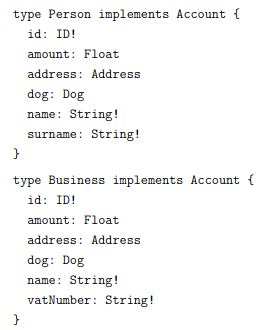
\includegraphics[scale=0.6]{Limits_Types.png}
                \end{figure}
                \column{0.6\textwidth}
                \begin{figure}
                    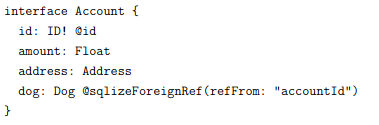
\includegraphics[scale=0.6]{Limits_Interface.png}
                \end{figure}
            \end{columns}
        \end{frame}

        \begin{frame}[plain,c]
            \begin{center}
                \huge Grazie dell'attenzione.
            \end{center}
        \end{frame}
\end{document}
